\documentclass[tikz,border=1pt]{standalone}
\input{figpreamble}
\begin{document}
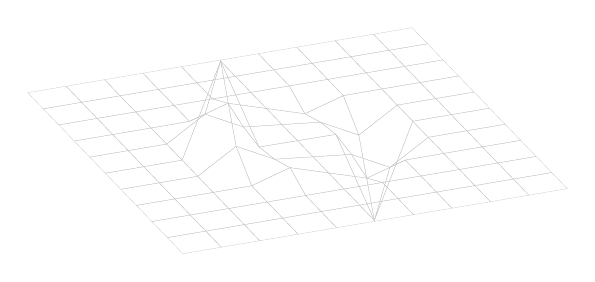
\begin{tikzpicture}[declare function={rr(\x,\y)=sqrt(\x*\x+\y*\y)+1e-9; sechsq(\a)=1/(cosh(\a)^2); fp(\r)=8*(sechsq(8*(\r+1)) - sechsq(8*(\r-1)))/(2*tanh(8));}]
\begin{axis}[hide axis, view={-22}{38}, colormap/viridis]
\addplot3[surf, shader=faceted, fill opacity=0, faceted color=black!22, line width=0.1pt, samples=11, samples y=11, domain=-2.6:2.6, y domain=-2.6:2.6, z buffer=sort] {x/rr(x,y)*fp(rr(x,y))};
\end{axis}
\end{tikzpicture}
\end{document}
